\section{Personalized Short-term Multi-Modal Interactions}
\label{sec:pers}
\vspace{-0.1cm}

As already mentioned, 
one of the main goals of the \coaches project is personalized short-term multi-modal interactions with non-expert users, that are typical customers of a shopping mall.

\begin{figure}
\centering
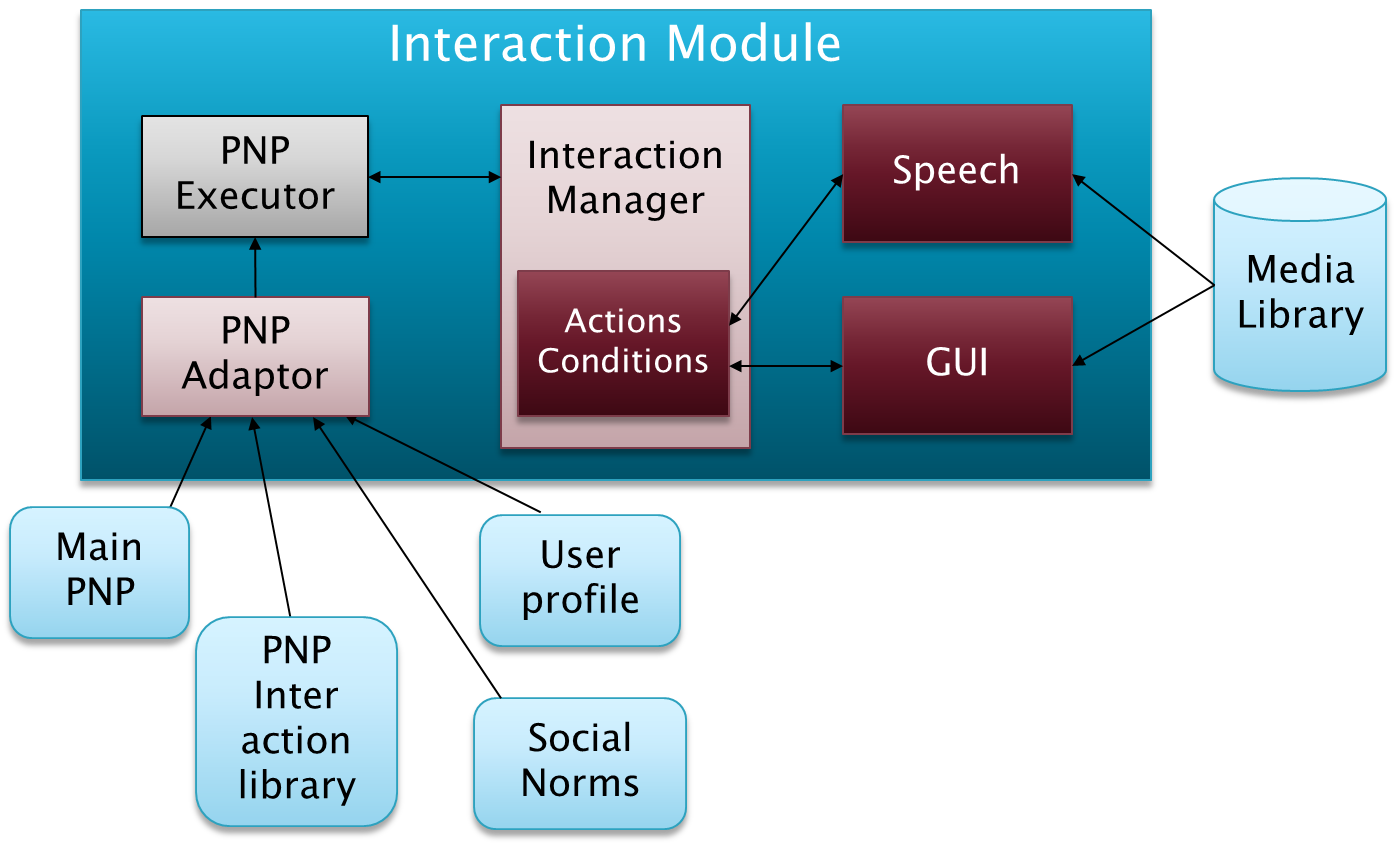
\includegraphics[width=0.9\textwidth]{fig/WP3.png}
\caption{Architecture of Interaction Module.}
\label{fig:WP3}
\end{figure}

The architecture of the Interaction Module is illustrated in Figure \ref{fig:WP3}. Data available to this module are Petri Net Plans (PNP) encoding the desired behavior of the robot, social norms, a user profile and a multi-media library.

The PNPs (as described later) encode the overall behavior of the robot, as generated by the planning and reasoning components of the system. The behavior include both basic robotic actions (e.g., moving in the environment) and interaction action.
The user profile are information available about the user that is interacting with the robot. %These data are in general not easy to obtain. %Since this is not the focus of this paper, we assume the data are available in an appropriate format acquired with appropriate means.
Among acquisition means for user profiles, it is possible to think about users wearing an RFID tag which contains personal information read by an RFID reader on-board the robot, or to the request of swiping a fidelity card, enter a personal password or showing to the robot a QR-code, in order to communicate to the robot the user profile.
In our implementation, we have used a simple identification mechanism based on recognizing QR-codes shown by the user to the robot on-board camera.

Finally, the media library is a collection of multi-media data (text, images, animations, video, etc.) that are linked to the communication activities of the robot and to the user profiles. We assume that in this library there are different versions of the same communication target for different users. For example, ice-cream advertisement can have a different spoken text and different displayed images or videos for children and adults.

In the remaining of this section, we will describe in more details the components of the interaction module.

\subsection{PNP Adaptor and Executor}

The Interaction Module is implemented within the framework of the Petri Net Plans (PNP) formalism \cite{ZiIo11PNP}. PNPs are based on two main concepts: \emph{actions} (i.e., output operations) and \emph{conditions} (i.e., input operations). Actions include motion of the robot in the environment, spoken sentences issued by the on-board speakers, text, images, videos or animations shown on the on-board screen, etc.
Conditions include the result of perception routines (e.g., image processing or speech recognition), the input given by a user through a GUI on the on-board screen, information about personal data of user acquired through a reader of fidelity cards, etc.

The use of PNPs for representing in an integrated way all these different kinds of actions and conditions allows for a strong coordination between the different sub-systems of the robot and for showing more complex behaviors and, in particular, a multi-modal interaction that can be easily customized according to the user.

The main plan, which include \emph{interaction plans} for HRI behaviors, generated by the reasoning and planning sub-system, is first processed by the PNP Adaptor and then executed by the PNP Executor. Both these modules are general-purpose, since all the relevant information is provided by external sources with an explicit representation. More specifically, the PNP Adaptor generates a personalized plan, given a main plan, a library of interaction plans, a set of social norms, and the user profile. The generated personalized plan is then executed by the PNP Executor. 
%While more details about this process are described in \cite{Io15}, in the rest of this section we illustrate its general concepts.

PNP Adaptor is implemented through an algorithm that transforms the Main PNP and the associated Interaction PNPs according to the social norms applied to the specific user profile. More specifically, the input plan is composed by a user-generic Main PNP that calls Interaction PNPs as sub-routines. All these plans are processed and transformed by applying the social norms (described as rules) customized to the current user profile.

The social norms are domain and task independent and are represented using a propositional logic formalism that follows the one described in \cite{BoPiTo09}. 
Given a set of propositions $U$ related to user profiles and a set of propositions $I$ related to forms of interactions, and given the set of formulas $U^{*}$ over $U$ and the set of literals $I^{+}$ over $I$,
a social norm is represented as a pair $(\phi,\delta) \in U^{*} \times I^{+}$, % or as a pair  $(\phi,a) \in L \times A$. $(\phi,\delta)$ has
with the meaning that if $\phi$ is true, then $\delta$ is mandatory (i.e., it must occur), or, in other words, $\neg \delta$ is forbidden. 
%$(\phi,a)$ has the meaning that if $\phi$ is true, then it is mandatory for the robot to execute the action $a$.

Some examples of social norms implemented in our system and considered in the examples in the next section are illustrated in Table \ref{tab:socialnorms}. 
%Actions are denoted with initial characters $A\_*$ to distinguish them from predicates. Note 

%\vspace{0.3cm}
\begin{table}
\begin{center}
\begin{tabular}{|l|} \hline
( child, use\_animation ) \\ 
( elder, use\_big\_font ) \\ 
( elder, use\_simple\_GUI ) \\
( deaf, $\neg$ use\_speech ) \\
( blind, $\neg$ use\_display ) \\
( elder $\vee$ deaf, display\_spoken\_text ) \\ 
( elder $\vee$ deaf $\vee$ blind, ask\_for\_guidance ) \\
( blind, use\_detailed\_speech ) \\
( blind, notify\_guidance ) \\
( first\_time\_user, detailed\_instructions ) \\ 
( $\neg$ first\_time\_user $\wedge$ young, $\neg$ detailed\_instructions ) \\ 
( child $\vee$ very\_young, $\neg$ use\_baby\_care\_room ) \\ 
( foreign, speak\_English ) \\ 
\hline
\end{tabular}
\caption{Domain-independent social norms.}
\label{tab:socialnorms}
\end{center}
\vspace{-0.8cm}
\end{table}
%\vspace{0.3cm}

Given a set of social norms $S$ and a user profile $u$ from which it is possible to determine the truth of the formulas in $U$, then it is possible to derive all the literals in $I^{+}$ that are implied by the social norms and $u$. In other words, it is possible to compute the set of propositions $\Delta_u$ such that $S \wedge u \models \Delta_u$. These propositions can be seen as the personalization of $S$ to $u$.
For example, if the user profile $u$ satisfies elder and deaf, $\Delta_u$ contains $\{$ use\_big\_font, display\_spoken\_text, use\_simple\_GUI, $\neg$ use\_speech $\}$. In this paper, we do not explicitly consider the case in which $\Delta_u$ may become inconsistent. Of course, several  mechanisms could be implemented for solving this issue, such as adding preferences or priorities to propositions.

The personalized propositions $\Delta_u$ affect the execution of the output actions of the interaction module. Each action in the PNPs is personalized by adding the appropriate propositions as arguments. As described later in the section, in this paper we consider two kinds of output interaction actions: \emph{Say}, related to the Speech module, and \emph{Show}, related to the Graphical Interface module.
Therefore, literals associated with \emph{Say} (e.g., $\neg$ use\_speech) are added as parameters of all the actions \emph{Say} in the PNPs, while literals associated with \emph{Show} (e.g., use\_big\_font, display\_spoken\_text, use\_simple\_GUI) are added as parameters of all the actions \emph{Show} in the PNPs.
These parameters determine the personalized interaction and will be considered by the Interaction Manager.

PNP Executor is a general-purpose executor of PNP already described in \cite{ZiIo11PNP} and successfully used in many applications. PNP Executor treats actions and conditions without giving them any semantics and controls only the flow of execution. The actual execution of the basic actions and conditions is responsibility of the Interaction Manager.

\subsection{Interaction Manager}
The interactions are coordinated by an Interaction Manager (IM), which manages all the robot activities (both the ones related with human-robot interaction and the ones used for implementing the basic robotic functionalities).
Its goal is thus to provide effective robot behaviors, including the personalized short-term multi-modal interactions described in this paper.

The IM is an action and condition server that executes actions and provides conditions, according to the requests of the PNP Executor module. It thus includes the definition of a set of primitive actions and conditions that are activated according to the plan under execution.
For the interaction behavior, actions and conditions are actually related to the Speech and Graphical Interface (GUI) modules described later. While the actions and the conditions related to the basic robot abilities (such as navigation, localization, perception, etc.) are not illustrated and described here, since the focus of this paper is on interaction.
The IM is also responsible to activate actions according to the personalized parameters defined by the PNP Adaptor module.

\subsection{Speech and Graphical Interfaces}

The interaction modalities considered so far in the project are speech and graphical interfaces.

\paragraph{Speech recognition and synthesis.}
The speech component allows the robot to communicate with humans through vocal interactions. 
It is formed by Automatic Speech Recognition (ASR) and Text-To-Speech (TTS).

The ASR component analyzes audio data coming from a microphone and extract semantic information about the spoken sentences, according to a predefined grammar. This component allows the robot to understand user spoken commands.
The speech recognition module is based on the Microsoft engine and on a further processing module that builds the semantic frames of the recognized sentences.
More details on the approach are available in \cite{BastianelliCCBN14}.

The TTS component transforms text messages in audio data that are then emitted by the speakers on-board the robot. This enables the robot to speak to people. The Microsoft TTS engine is used for this module.


\paragraph{Graphical User Interface.}

The GUI component implements a graphical input and output interface between users and robots that is displayed through the touch screen on-board the robot. The GUI defines actions (i.e., output operations) and conditions (i.e., input operations) that are integrated in the IM with other communication primitives (e.g., speech) in order to implement a multi-modal interaction.

\vspace{0.3cm}
The Speech and GUI components make available to the IM the implementation of actions and conditions that are executed according to the PNPs. These are summarized in the following table.
\vspace{1em}
\begin{center}
%\begin{table}
\begin{tabular}{|c|c|c|} \hline
 & {\bf Action} & {\bf Condition} \\  \hline
Speech & 
\begin{tabular}{c}
\emph{Say} \\ 
speak information though TTS
\end{tabular} & 
\begin{tabular}{c}
\emph{ASR} \\ 
Results of ASR
\end{tabular} \\ \hline
GUI & 
\begin{tabular}{c}
\emph{Show} \\ 
show information on the GUI
\end{tabular} & 
\begin{tabular}{c}
\emph{GUI} \\ 
Results of GUI input
\end{tabular} \\ \hline
\end{tabular}  
%\label{}
%\caption
\end{center}
\vspace{0.3cm}

The actions implemented at this level are parametric with respect to a set of parameters expressed as propositions and used to define the social norms. As mentioned above, during the process, general actions are associated to specific parameters depending on the user profile. This parameters are considered to specialize the execution of the actions. Two kinds of specializations are considered: 1) modification of some internal parameters of the action (for example, the size of the font in a displayed text), 2) selection of the proper media to communicate.
The second specialization is related to the presence of multiple options in the Media Library for the same communicative target. In these cases, each option is labeled with a precondition using the same interaction propositions in $I$. Therefore, it is possible to select appropriate media considering the personalized propositions $\Delta_u$.



